\documentclass{article}
\usepackage[utf8]{inputenc}
\usepackage{graphicx}
\usepackage{xcolor}

\begin{center}
\textbf{\Large{Shri G.S Institute of Technology and Science}}\\
\vspace{5pt}
\textbf{CO24497 : PROGRAMMING PRACTICES}\\
\vspace{5pt}
\textbf{Mini project}
\begin{flushright}
November-2022 \\
\end{flushright}
\end{center}
\begin{center}
\LARGE{\underline{Project Report}}\\
\end{center}

\begin{document}


\section{Objective of Project:-}

$\bullet${ This mini project is just a basic guide for C language.}\\
$\bullet${It's just a try to make it user-friendly with the best possible indentation to make it as much as visible.}\\
\vspace{10pt}
$\color{blue}{\\
\textit{\underline{Included Chapter:-}}}${\\
$\bullet$  Header Files in C\\
$\bullet$  Basic Syntex\\
$\bullet$  How to print\\
$\bullet$  Different types of Data-Types\\
$\bullet$  Reserved Key-words\\
$\bullet$  Operators\\
$\bullet$  Arrays\\
$\bullet$  Loops\\
$\bullet$  Pointer\\
$\bullet$  Funtions\\
$\bullet$  Practice Sets\\}
\\$\color{cyan}\textbf{ The main objective of this mini project is to make users familiar with C language......}$
\section{Function Description:-}
There are 11 functions,8 sub-functions, and 1 main function\\{\hspace{15pt}Each function is defined as a Unique chapter.}\\\\
{\color{red} Chapter-1:- Header files in C\\}
$\bullet$ It includes all header files.\\
{\color{red}Chapter-2:- Basic Syntax \\}
$\bullet$ This chapter describes the basic syntax and all needed information required for C.\\
{\color{red}Chapter-3:- How to print \\}
$\bullet$ This chapter describes how c language prints giving data terminal.\\
$\bullet$ In this chapter there are three methods for printing in C.\\
{\color{red}Chapter-4:- Different types of Data-Types\\}
$\bullet$ This chapter describes different types of data types.\\ 

{\pagebreak}

{\color{red}Chapter-5:- Reserved Key-words}\\
$\bullet$ In this chapter there is the list of reserved keywords \\
$\bullet$ Reserved key word are those keywords which can't be used for declaration name for datatype. \\
{\color{red}Chapter-6:- Operators}\\
$\bullet$ In this chapter all kind of operator that are used in c is discussed.\\
{\color{red}Chapter-7:- Arrays}\\
$\bullet$ In this chapter definition and declaration of arrays are discus.\\
{\color{red}Chapter-8:- Loops}\\
$\bullet$ There are three kind of loops that is For loop,While loop,do-While loop all are disscus in this chapter.\\
{\color{red}Chapter-9:- Pointers}\\
$\bullet$ Different kinds of defination and its part are define in this chapter.\\
{\color{red}Chapter-10:- Functions}\\
$\bullet$ How can we use function in C are define here .\\
{\color{red}Chapter-11:- Practice-set}\\
$\bullet$ It's just a implementation of above chapters.....\\
\section{GDB screen shoots :-}
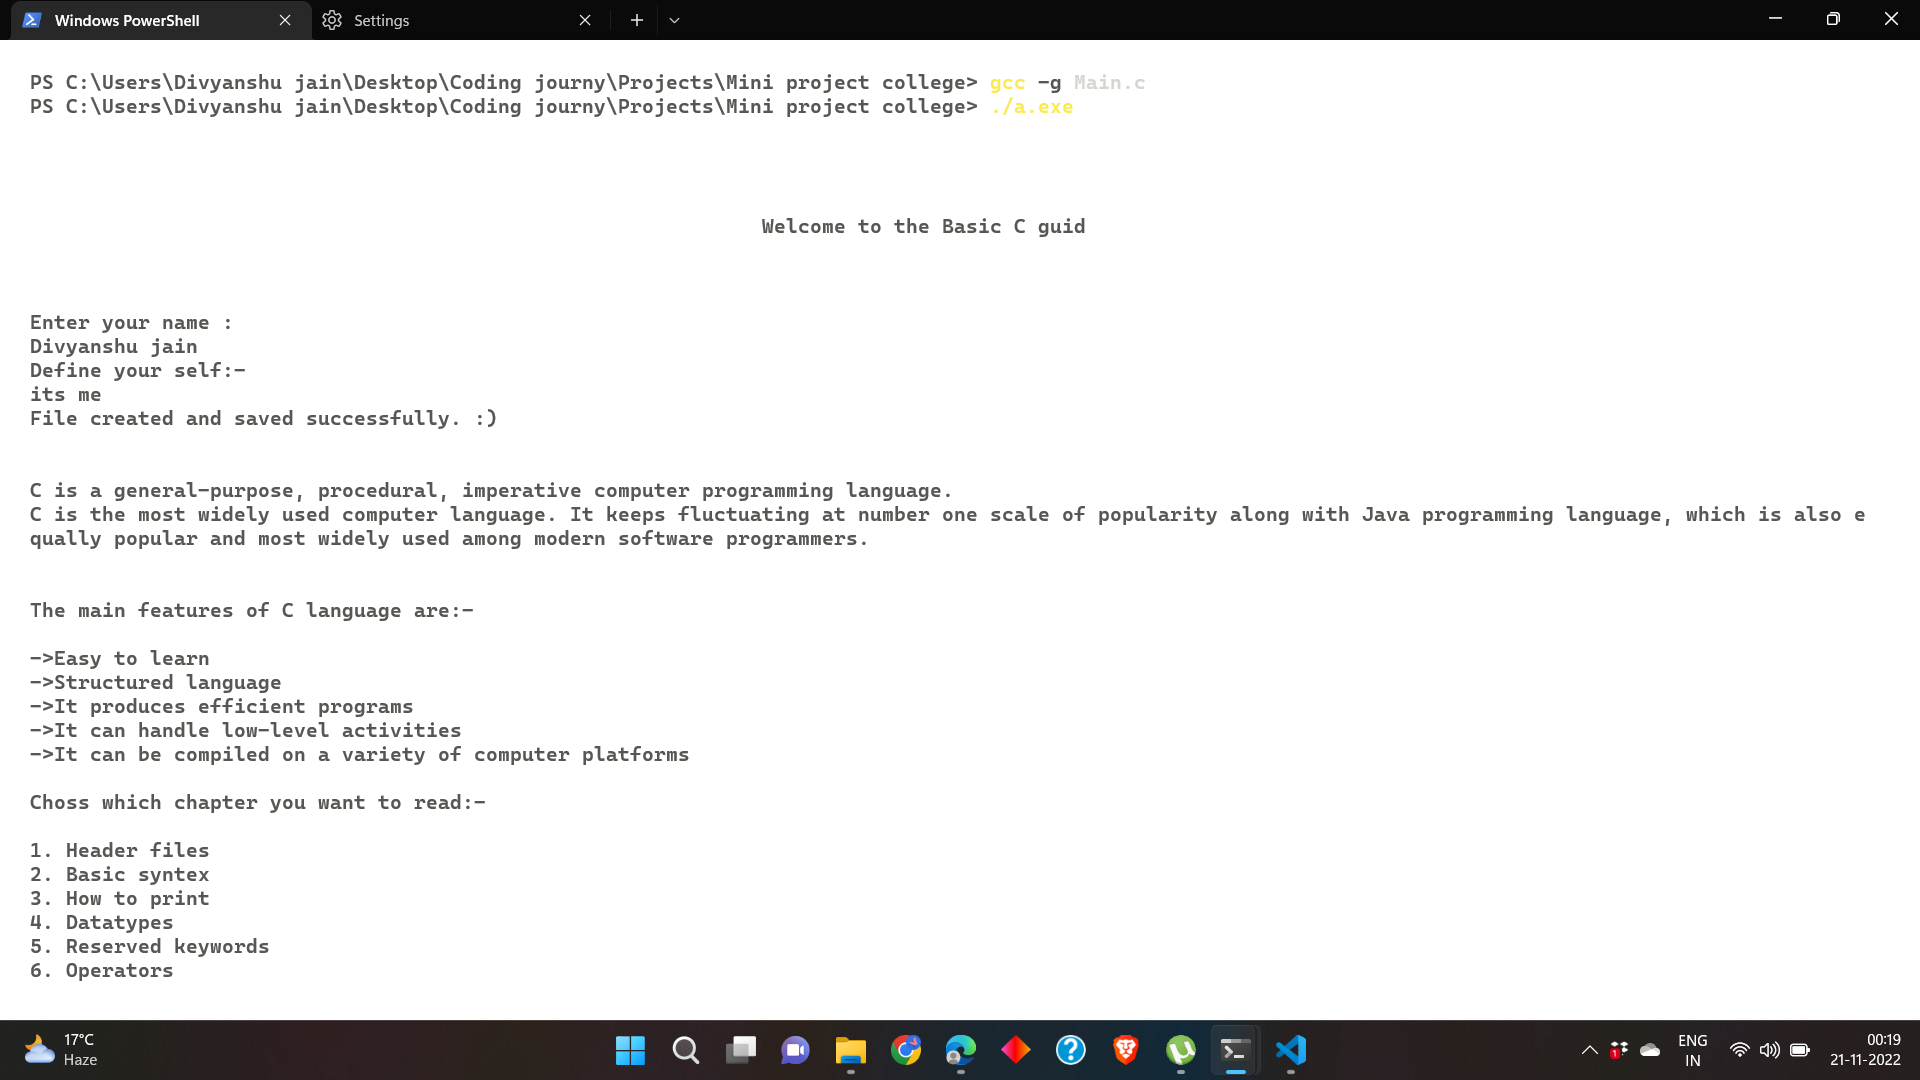
\includegraphics[width=\linewidth]{pic1.png}\\
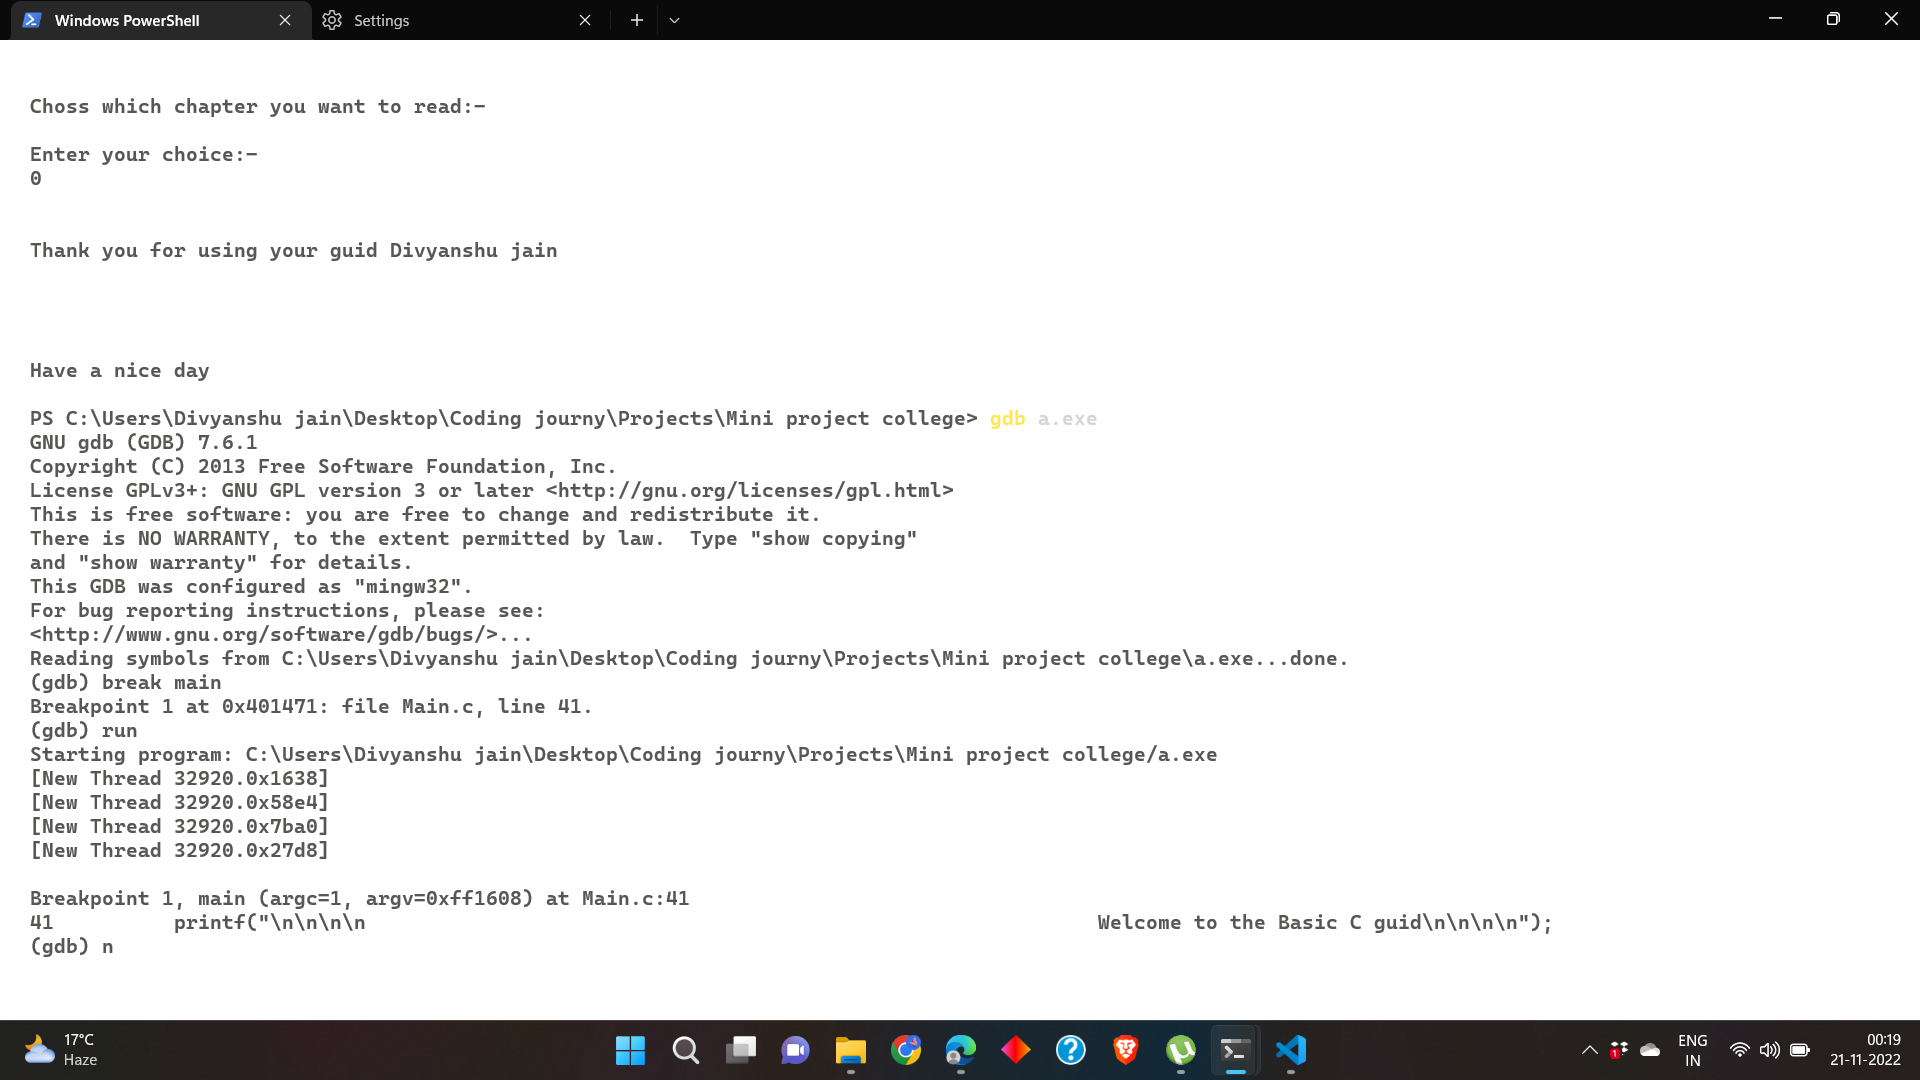
\includegraphics[width=\linewidth]{pic2.png}\\
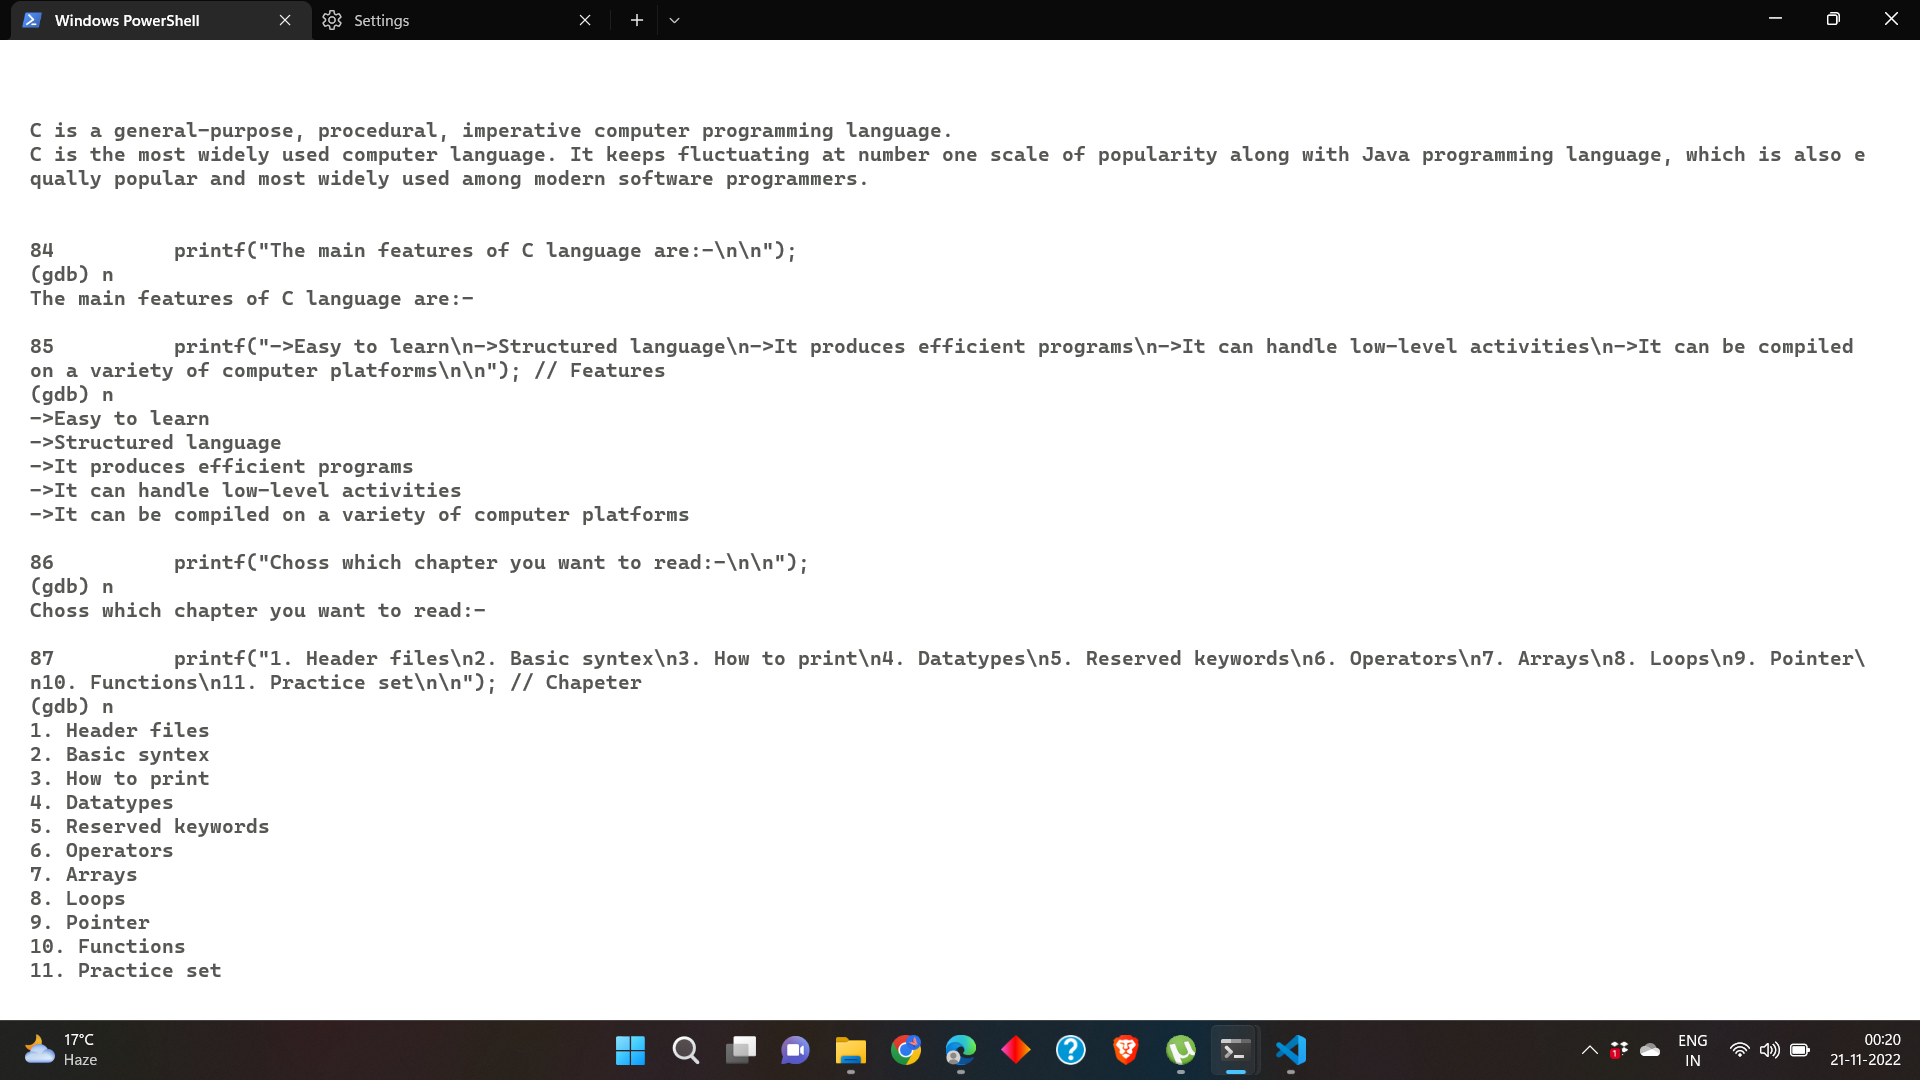
\includegraphics[width=\linewidth]{pic3.png}\\
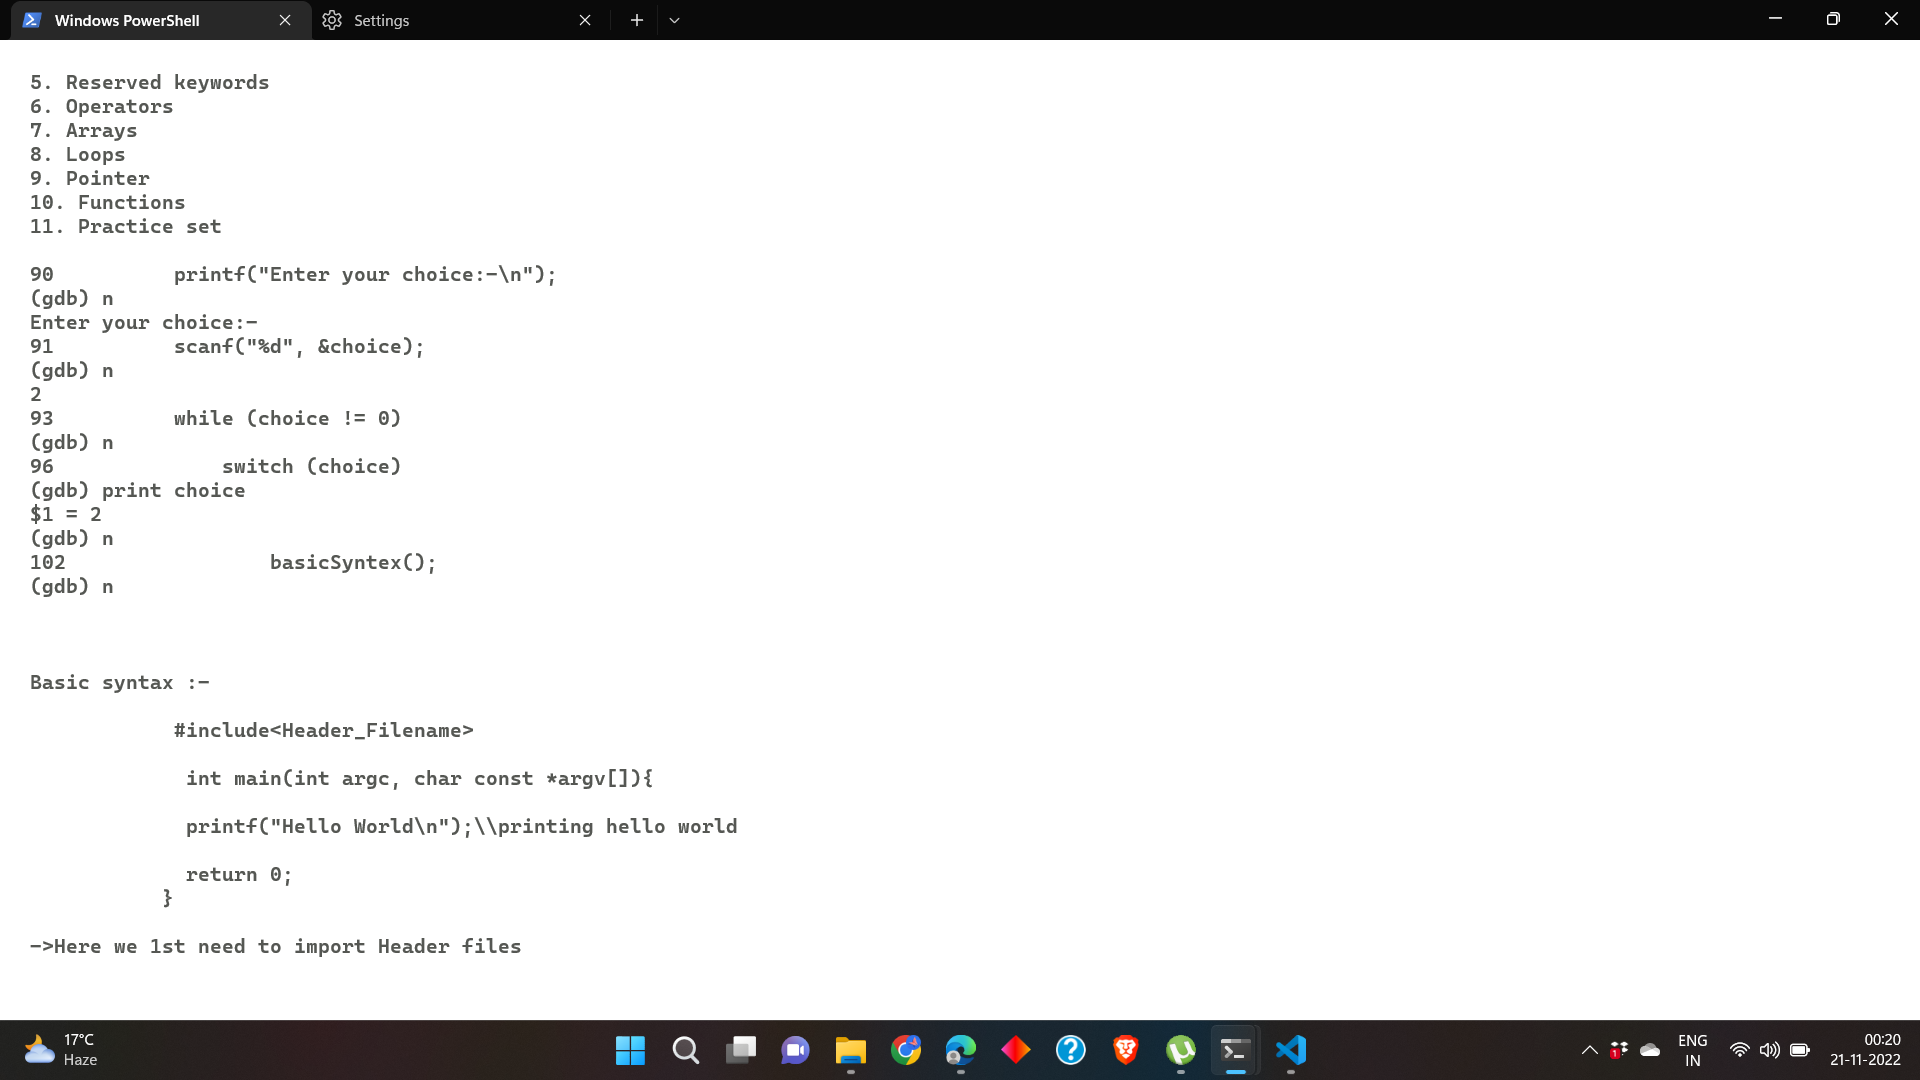
\includegraphics[width=\linewidth]{pic4.png}\\
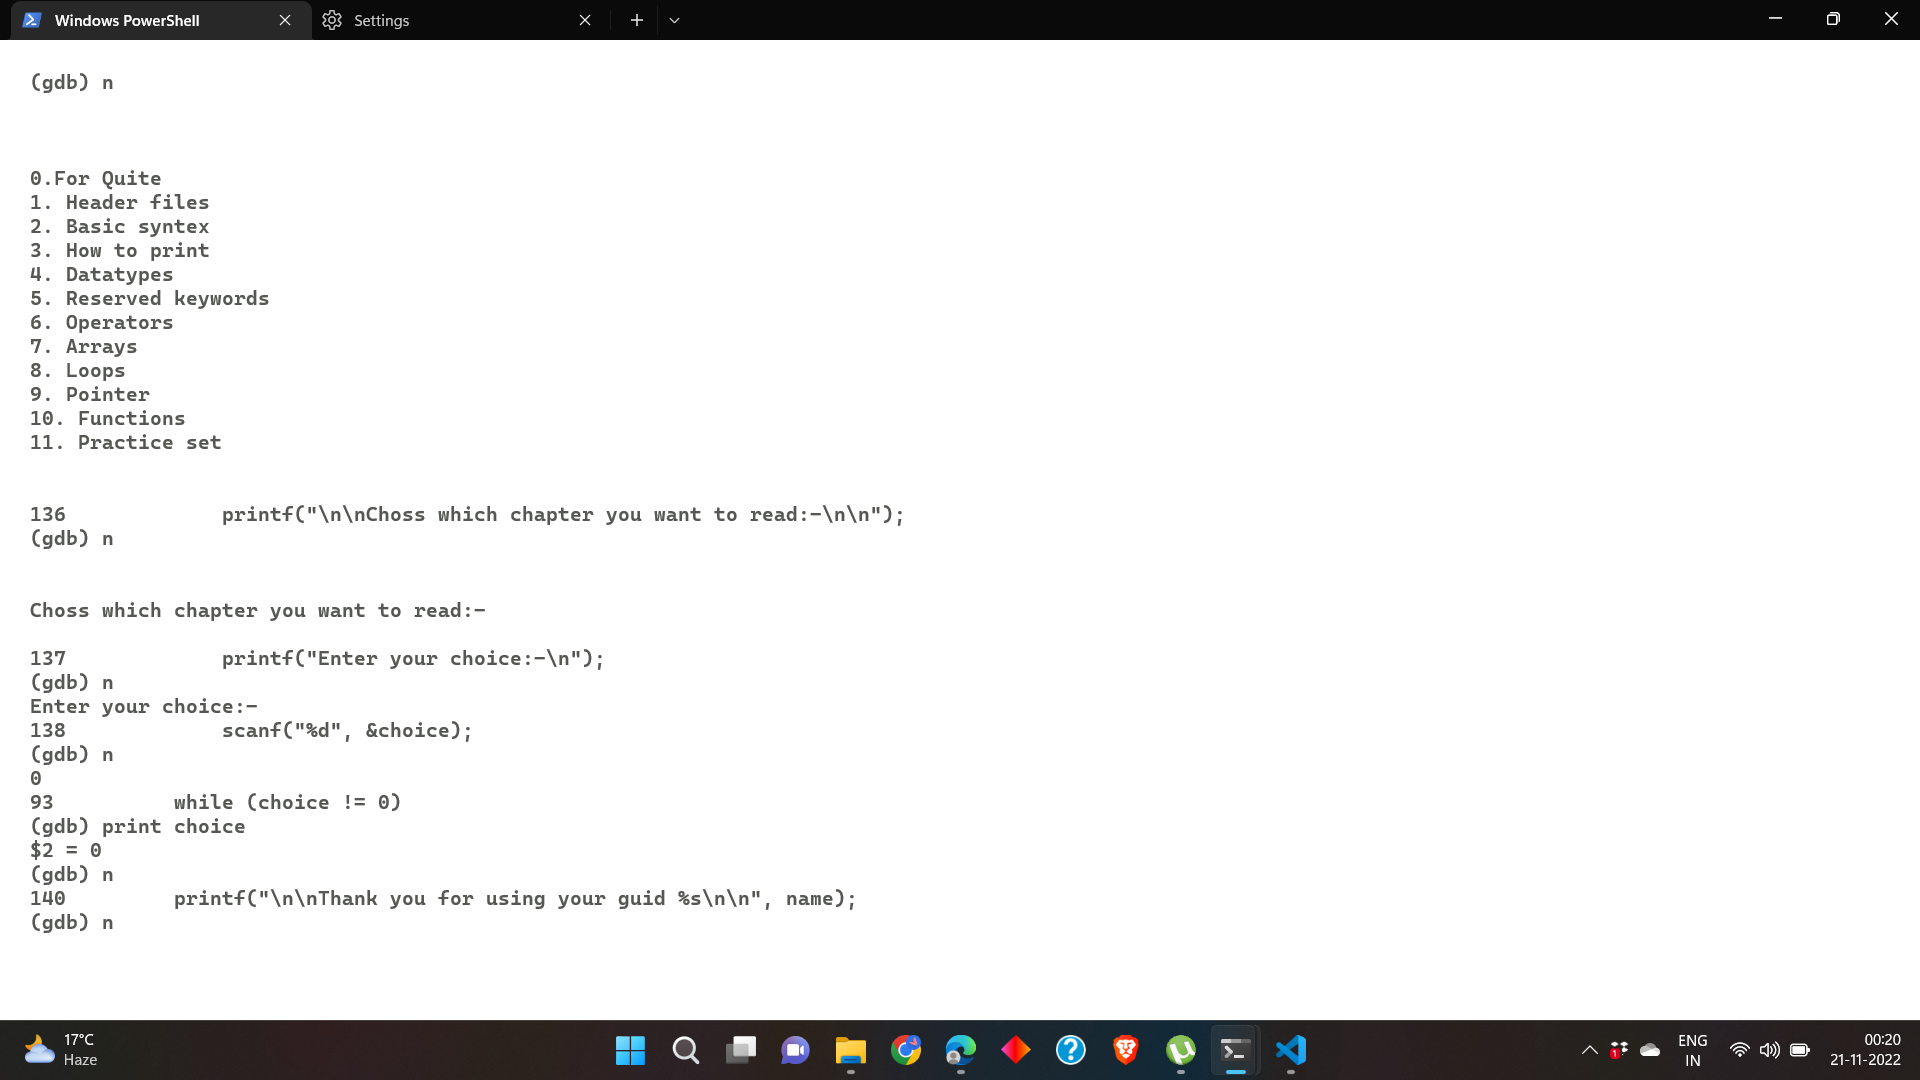
\includegraphics[width=\linewidth]{pic5.png}\\
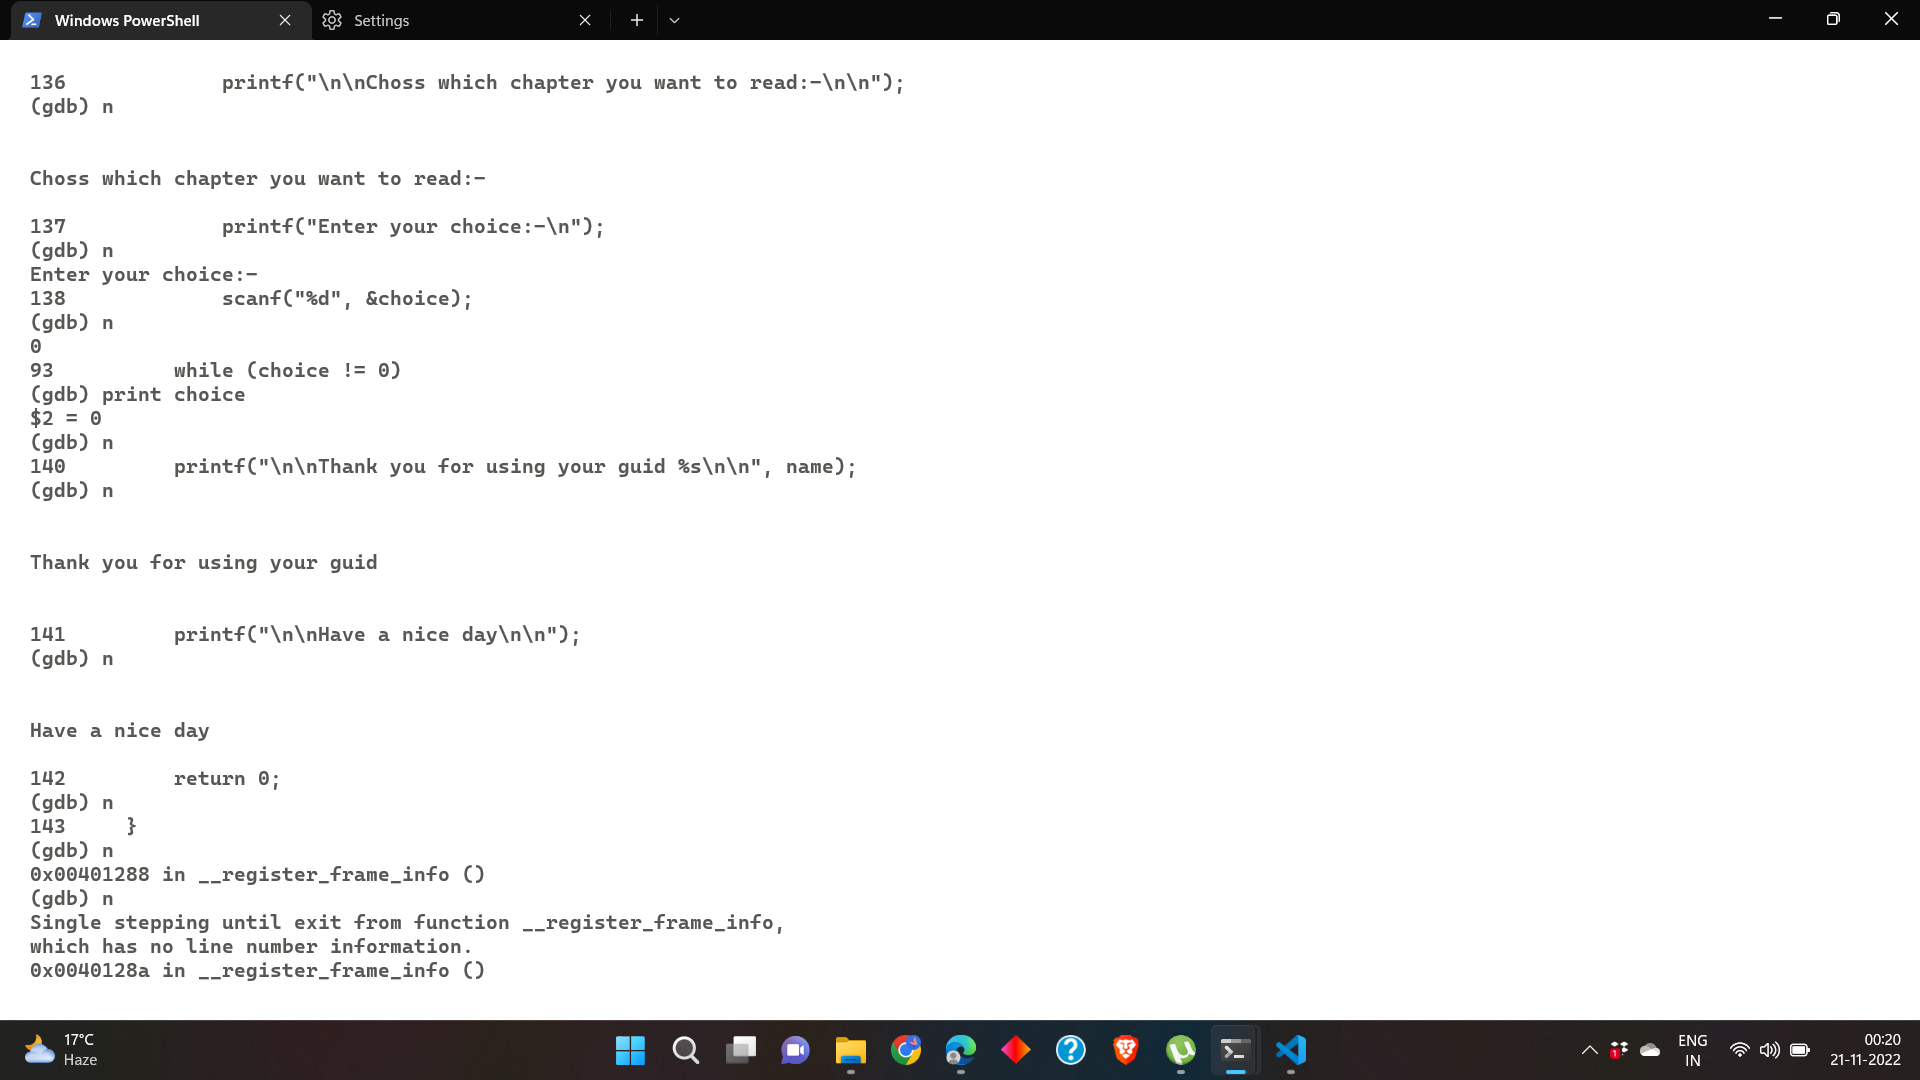
\includegraphics[width=\linewidth]{pic6.png}\\




















\end{document}
